\chapter{Implementazione}
In questo capitolo viene discusso come sono stati implementati i moduli e gli algoritmi precedentemente introdotti.
Vengono illustrate le scelte implementative che sono state prese e le tecnologie utilizzate.

Il linguaggio scelto per lo sviluppo del sistema, a parte l'interfaccia grafica, è Erlang, un linguaggio per lo sviluppo concorrente che può essere usato anche
per sviluppare sistemi distribuiti ed il set di librerie \textit{OTP}.  Offre nativamente varie librerie per la creazione di processi e nodi e per la loro comunicazione.
Inoltre, Erlang gestisce automaticamente la connessione tra nodi, se un nodo si connette ad un'altro, il primo sarà automaticamente connesso anche a tutti i nodi
a cui è connesso il secondo. In questa maniera non serve implementare un algoritmo di routing e mantenere uno spanning tree dei nodi.

\section{Ant Colony}

\section{Ant Colony Optimization}

\section{Comunicazione}
La comunicazione tra nodi e processi è offerta e gestita dal linguaggio e dalle librerie \texttt{OTP},
quindi non è stato necessario implementarle.

\section{Ticket System}
Il ticket system è stato implementato con due moduli, \texttt{ticket\_system}, che ne offre le API,
e \texttt{ticket\_system\_server} che ne gestisce le funzionalità.

Il modulo \texttt{ticket\_system\_server} è implementato con un behaviour \texttt{gen\_server} di \texttt{OTP}.
Si occupa di due funzionalità, gestire i ticket ed eleggere il ticket master.
L'elezione è implementata seguendo l'algoritmo descritto in \ref{sub:tm_ele}, usando un \texttt{handle\_call} e tre \texttt{handle\_cast}.
La call viene utilizzata per far partire l'elezione e poter rispondere con l'id del leader e confermare il successo dell'operazione.
Una volta che l'iniziatore ha ricevuto la call, fa partire l'echo del suo id tramite un \texttt{gen\_server:abcast} a tutti gli altri
nodi del sistemi, che lo riceveranno ed eleboreranno con un \texttt{handle\_cast}. 
Gli step sono descritti nel capitolo precedente, con i messaggi di \texttt{{ok, Leader}} gestiti da un altro
\texttt{handle\_cast}. Ogni processo ho poi uno stato, dove registra il proprio leader corrente e quanti messaggi con lo stesso
leader ha ricevuto, per adedire allo step \ref{ticket:ok_step}. Ultimo elemento dello stato è \texttt{status}
che serve al processo per sapere se è o meno l'iniziatore dell'echo corrente. Nel caso in cui lo fosse
e ha ricevuto tutti i messaggi necessari, allora si può considerare eletto. I messaggi dell'elezione terminano
e il leader risponde al processo che ha chiesto l'elezione tramite una chiamata di \texttt{gen\_server:reply}.
Infine, per evitare possibili errori con l'interazione con il sistema ant colony, il leader deve impostare
il valore del prossimo ticket da dispensare. Per fare ciò, chiede a tutti i processi \texttt{aco\_node} quale sia
stato l'ultimo ticket da loro elaborato, prendendo quello maggiore tra le risposte ricevute.

Il modulo offre anche la funzionalità per collegarsi al ticket system dopo che questo è già partito
e ha eletto un leader, con la chiamata \texttt{connect} tramite un \texttt{gen\_server:call}.

Le funzionalità per far partire l'elezione, chiedere chi sia il ticket master e richiedere un nuovo ticket sono
rese disponibili dal modulo \texttt{ticket\_system} che gestisce anche la possibilità che il leader sia crashato
o non più responsivo.
\section{User}
Il modulo \texttt{user\_node} è l'intermediario tra le API utente e il sistema, ed è anch'esso implementato con il 
behaviour \texttt{gen\_server} di \texttt{Erlang/OTP}.

Il modulo ha uno stato in cui mantiene una lista di coppie (ID ufficio - ID nodo), che aggiorna ogni qual volta venga
aggiunto un nuovo officio.

Nel caso in cui il processo si unisce ad un sistema già in corso, tramite la call \texttt{connect} inizia il processo
di inviare a tutti i nodi la propria lista e di ricevere in risposta le liste di tutti gli altri nodi, in modo da
sapere tutti gli uffici presenti.

Per ogni chiamata che si occupa di modificare lo stato del grafo dei clienti, il modulo inizia chiedendo
al ticket master un biglietto, usando \texttt{ticket\_system:request\_ticket()}. Dopodichè esegue la call corretta e 
informa i processi \texttt{aco\_node} di aggiornare il ticket (se necessario), usando la call \texttt{update\_ticket}.
Infine risponde al processo chiamante con un messaggio di successo o fallimento, in base al risultato delle chiamate.

\section{User API}
Le API utente sono implementate con il modulo \texttt{user\_api}.
Il sistema offre diversi metodi, divisi in due categorie: interazioni con il sistema e setup.

La prima categoria offre i seguenti metodi, tutti implementati con 
\texttt{gen\_server:call} al processo \texttt{user\_node}:
aggiunta e rimozione di clienti, aggiunta e rimozione di uffici, aggiornamento dei costi.

La seconda categoria offre invece i metodi necessari per eseguire il setup del sistema:
aggiunta iniziale di clienti e dei costi, avvio dei processi necessari e avvio del sistema.
Per l'avvio dei processi sono stati implementati due metodi, il primo offre l'avvio di tutti i processid
usati dal sistema: \texttt{aco\_node, user\_node, ticket\_system\_server} e \texttt{flooding}. Il secondo
invece implementa l'avvio soltanto dei due processi necessari per il corretto funzionamento di un nodo, \texttt{aco\_node} e \texttt{ticket\_system\_server}.
Quest'ultimo non permette al nodo di interagire con il sistema con la prima categoria di API utente.

\section{Flooding}\label{sec:flood}
Il modulo di flooding è implementato con un semplice behaviour \texttt{gen\_server}, offerto da
\texttt{Erlang/OTP}. Il modulo ha due funzioni principali:
scrivere su file una rappresentazione xml del grafo clienti e scrivere una rappresentazione xml dei percorsi effettuati dalle formiche.

La prima funzione è implementata da \texttt{write\_graph\_to\_file()} che chiede ai processi \texttt{aco\_node} di tutto il sistema
i propri nodi e archi, li mette insieme e li stampa su file. Per l'elaborazione dei dati XML viene usata la libreria \texttt{XMERL}.

La seconda funzione viene chiamata ogni qualvolta che una formica finisce un percorso. Il processo \texttt{aco\_node} fa un \texttt{gen\_server:cast} al processo
\texttt{flooding} con i dati del percorso effettuato. Appena viene ricevuto il messaggio, il percorso viene elaborato in un elemento XML ed inserito
nel file dei percorsi.


\section{Interfaccia Grafica}
\begin{figure}
    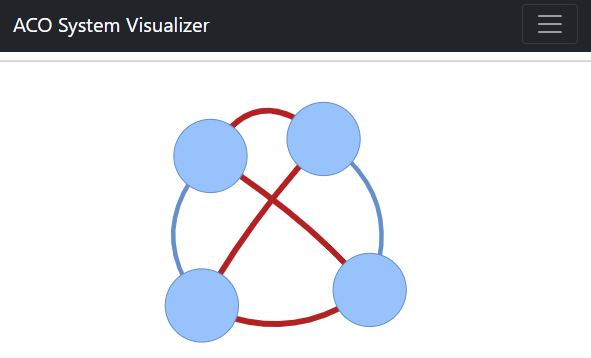
\includegraphics[width=\textwidth]{images/gui.png}
    \centering
    \caption{Esempio dell'interfaccia grafica}
    \label{fig:gui}
\end{figure}

 Per implementare l'interfaccia grafica richiesta è stato deciso di utilizzare una webapp, per poter permettere facilmente l'accesso al servizio
 da una moltitudine di dispositivi diversi. Per realizzare la suddetta webapp è stato scelto di utilizzare Flask \cite{flask}, un microframework scritto in python.
 Flask offre un web server leggero e semplice da utilizzare, che permette di accedere all'enorme repertorio di librerie di Python.

 Per visualizzare il grafo e il percorso migliore è stato optato di utilizzare la libreria PyVis \cite{Pyvis}.
 Questa libreria offre la visualizzare, fornita da un file html, di un grafo e di potervi interagire, spostando i nodi e gli archi tramite il cursore.
 Offre inoltre una buona gamma di opzioni grafiche, tra cui poter dare un nome ad un nodo o un arco, modificare il colore di un elemento e modificare la dimensione.
 
 Come scritto per il modulo flooding in sezione \ref{sub:flood}, vengono utilizzati due file XML per comunicare alla GUI i dati del grafo e dei percorsi trovati.
 Per parsare i file XML in Python viene utilizzata la libreria \texttt{xml.minidom}. Non sono state fatte richieste su requisiti di sicurezza ma tale libreria è vulnerabile
 a due attacchi, \texttt{Billion Laughs} \cite{BillionLaughs} e \texttt{Quadratic Blowup} \cite{QuadBlow}. In quanto i file XML sono generati da una fonte fidata, ovvero il
 sistema stesso, non dovrebbero poter venir usati. Nel caso in cui un'entità esterna riuscisse a modificare i due file, allora il sistema diventerebbe suscettibile ai due attacchi.

 In futuro si dovrebbe cambiare usando \texttt{json} o \texttt{yaml}.

 Il frontend dell'interfaccia è invece realizzato usando \texttt{Bootstrap}.

 In figura \ref{fig:gui} è possibile vedere un esempio dell'interfaccia grafica. Il percorso migliore viene evidenziato in rosso e ne viene comunicato il costo.

 L'interfaccia si aggiorna autonomamente ogni 30 secondi, per poter dare sempre le informazioni più recenti.

 I metodi per la gestione del web server sono racchiusi in \texttt{app.py} e si occupano di renderizzare
 i template HTML, a parte \texttt{update()}. Questo metodo viene chiamato dal frontend tramite \texttt{javascript} ogni 30 secondi
 e legge i file XML del grafo e dei percorsi e ricrea la visualizzazione.
 La gestione del grafo visualizzabile è fatta da \texttt{backend.py} che comprende i metodi per aggiungere 
 nodi e archi e sottolineare il percorso migliore. Quest'ultimo viene estrapolato dai dati di tutti i percorsi,
 cercando il percorso con il costo minore e lo stesso insieme di nodi dell'ultimo percorso registrato, con la funzione
 \texttt{drawBestPath()}.
